\documentclass[12pt,a4paper]{report}
\usepackage[utf8]{inputenc}
\usepackage[spanish]{babel}
\usepackage{amsmath}
\usepackage{amsfonts}
\usepackage{amssymb}
\usepackage{makeidx}
\usepackage{graphicx}
\usepackage[hidelinks]{hyperref}
\usepackage[left=2cm,right=2cm,top=2cm,bottom=2cm]{geometry}
\usepackage{hyperref}



\begin{document}

\author{Fonseca Camarena Jonathan}

\title{\begin{center}

\includegraphics[scale=1.5]{Escudo.png} 
\end{center}Explicar la convención Denavit-Hartenberg}

\date{
Universidad Politécnica de la Zona Metropolitana de Guadalajara\\
Profesor: Carlos Enrique Morán Garabito\\
24 de septiembre del 2019}

\maketitle
\tableofcontents
\section{Introducción}
Se trata de un procedimieto sistemático para describir la estructura cinemática de una cadena articulada
constituida por articulaciones con. un solo grado de libertad.
Para ello, a cada articulación se le asigna un Sistema de Referencia Local con origen en un punto Qi
 y ejes
ortonormales { X Y Z i i i , , } , comenzando con un primer S.R fijo e inmóvil dado por los ejes { X Y Z 0 0 0 , , } ,
anclado a un punto fijo Q0
 de la Base sobre la que está montada toda la estructura de la cadena.
Este Sistema de Referencia no tiene por qué ser el Universal con origen en (0,0,0) y la Base canónica.
\section{Sistema de Referencia}
Para comenzar hay que entender que este convenio para definir parámetros es una simplificación de la descripción cinemática de un sistema en el que intervienen una serie de articulaciones.
Supongamos un brazo que puede girar el hombro y el codo hasta la muñeca. Pues para mover la muñeca hasta una posición indicada es evidente que hay que mover las articulaciones anteriores desde el hombro que ha de levantar el codo y finalmente nuestra mano para poder saludar al vecino. A esto se le llama cinemática directa ya que existe una jerarquía de movimientos en la que el padre dominante es el hombro, y el codo y la muñeca sus hijas. Y de la misma manera el codo es padre de la muñeca.\\
\noindent\\
En fin, esta cinemática está gobernada por la denominada composición de movimientos que de forma simple permite conocer como se mueve un punto B (codo) de nuestro brazo, conociendo el movimiento de otro punto A (hombro) y la relación de giro o traslación que hay entre ellos. De esta manera, si sabemos como se mueve el punto B (codo) que pertenece a otro eslabón (en este caso el antebrazo), podremos saber, como se mueve el punto C que es nuestra muñeca.\\
Pues con este ejemplo se puede aplicar la misma transformación a otro diseño de brazo y de manera sucesiva se pueden conocer todas las variables cinemáticas para ir más allá en robótica.\\
La mecánica clásica establece una serie de ecuaciones en la que se considera una referencia fija; en nuestro caso el hombro si suponemos que estamos parados; y otra referencia móvil que son las articulaciones siguientes. Por ello, hay que diseñar una serie de referencias con sus ejes (x,y,z) en cada articulación y siguiendo las instrucciones que indica el convenio de Denavit-Hartenberg, definir 4 parámetros que las relacionan.\\


\begin{figure}
  \centering
    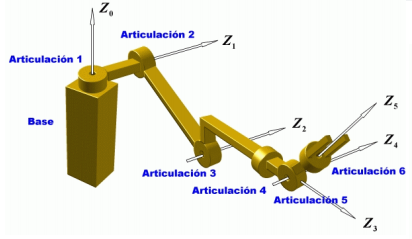
\includegraphics{Robot.png}
  \caption{Brazo}
  \label{fig:Tabla}
\end{figure}


\section{Rotacionales o Prismatica}
Las articulaciones pueden ser rotacionales o prismáticas, osea que giran o se trasladan en una dirección. Y cada una de estas articulaciones sea del tipo que sea provee al sistema de un grado de libertad adicional. Y es recomendable no superar los 6 grados de libertad si se es inexperto.\\


\begin{figure}
\centering
  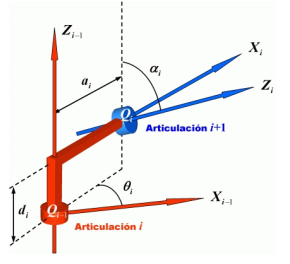
\includegraphics[scale=.5]{Robot1.png}\\
    Figura 2:Rotaciones.
\end{figure}

\section{Articulaciones compuestas con 2 o 3 Grados de libertad}
Un caso muy frecuente es el de las articulaciones del cuerpo humano o de un animal en el que un hueso
puede girar respecto al anterior en 2 o 3 ejes que se cortan en un mismo punto y más aún, podemos suponer
que los ejes son mutuamente perpendiculares.
Cada uno de estos ejes de rotación constituye una articulación en el sentido de la representación DenavitHartenberg, pero para esta situación especial resulta conveniente cambiar la notación vista en la sección
anterior y denominar a los Sistemas de Referencia como:


\centering
  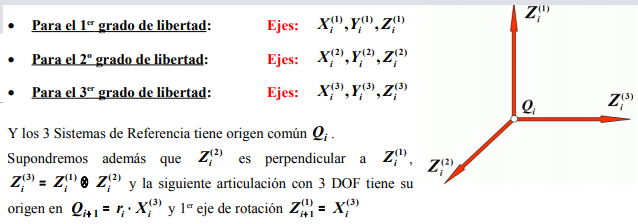
\includegraphics[scale=.5]{Robot2.png}\\
    Figura 2:Grados de Libertad.


\section{Referencia}


\cite{del2011representacion}

\bibliographystyle{unsrt}
\bibliography{Biblio}




\begin{center}
Gracias.
\end{center}


\end{document}